%\documentclass[11pt]{article}
\documentclass{clv2}
\issue{?}{?}{2012}

%Document Head
\dochead{Draft Paper \date{}}

\runningtitle{Learning Syntactic Categories Using Paradigmatic
  Representations of Word Context}

\runningauthor{?}

%\usepackage{acl2012}
\usepackage{times}
\usepackage{latexsym}
\usepackage{amsmath}
\usepackage{multirow}
\usepackage{url}
\usepackage{graphicx}
\usepackage{pdflscape} %% Better readable
%\usepackage{lscape}
%%% DY: Some consistency macros:

% many-to-one abbreviation
% 429 uses MTO
% Lamar uses M-to-1
% Maron uses MTO
% Lamar uses MTO
% Let us go with MTO
\newcommand{\mto}{\mbox{MTO }}

% Let us go with VM for V-measure
\newcommand{\vm}{\mbox{VM }}

% Adopt the .7654 convention rather than percentages like 76.54%.
% Define the results here for consistency
\newcommand{\bgmto}{.7314 (.0096)}
\newcommand{\bgvm}{.6558 (.0052)}
\newcommand{\rpmto}{.7554 (.0055)}
\newcommand{\rpvm}{.6703 (.0037)}
\newcommand{\wsmto}{.7680 (.0038)}
\newcommand{\wsvm}{.6822 (.0029)}
\newcommand{\ftmto}{.8023 (.0070)}
\newcommand{\ftvm}{.7207 (.0041)}

\title{Learning Syntactic Categories Using Paradigmatic
  Representations of\\ Word Context}

\author{
%Mehmet Ali Yatbaz \hspace*{10mm} Enis Sert \hspace*{10mm} Deniz Yuret \\
%Artificial Intelligence Laboratory \\
%Ko\c{c} University, \.Istanbul, Turkey \\
%\{myatbaz,esert,dyuret\}@ku.edu.tr
}
\begin{document}
\maketitle
%%

\section{Introduction}
\label{sec:intro}

Grammar rules apply not to individual words (e.g. dog, eat) but to
syntactic categories of words (e.g. noun, verb).  Thus constructing
syntactic categories (also known as lexical or part-of-speech
categories) is one of the fundamental problems in language
acquisition.

Linguists identify syntactic categories based on semantic, syntactic,
and morphological properties of words.  There is also evidence that
children use prosodic and phonological features to bootstrap syntactic
category acquisition \cite{ambridge2011child}.  However there is as
yet no satisfactory computational model that can match human
performance.  Thus identifying the best set of features and best
learning algorithms for syntactic category acquisition is still an
open problem.

Computational models of syntactic category acquisition in the
literature mainly rely on distributional analysis: Items that share
the same distribution (i.e. that occur in the same context) are
grouped into the same category.  The definition of ``the same
context'' vary across studies.  Algorithms based on the Hidden Markov
Model use class based n-grams to specify context
\cite{Brown:1992:CNG:176313.176316}, others use a frame of neighboring
words around the target word \cite{Schutze:1995:DPT:976973.976994}.
Our main contribution in this study is to introduce paradigmatic
features, i.e. features based on potential substitutes of the target
word, to represent word context.

Relationships between linguistic units can be classified into two
types: syntagmatic (concerning positioning), and paradigmatic
(concerning substitution).  Syntagmatic relations determine which
units can combine to create larger groups and paradigmatic relations
determine which units can be substituted for one another.
Figure~\ref{fig:paradigmatic} illustrates the paradigmatic vs
syntagmatic axes for words in a simple sentence and their possible
substitutes.

\begin{figure}[h] \centering
% Generated with LaTeXDraw 2.0.8
% Tue Jan 10 15:57:06 EET 2012
% \usepackage[usenames,dvipsnames]{pstricks}
% \usepackage{epsfig}
% \usepackage{pst-grad} % For gradients
% \usepackage{pst-plot} % For axes
\scalebox{1} % Change this value to rescale the drawing.
{
\begin{pspicture}(0,-1.6728125)(4.73474,1.6528125)
\usefont{T1}{ptm}{m}{n}
\rput(0.39520833,-0.6571875){\psframebox[linewidth=0.04]{the}}
\usefont{T1}{ptm}{m}{n}
\rput(1.8816146,-0.6571875){\psframebox[linewidth=0.04]{man}}
\usefont{T1}{ptm}{m}{n}
\rput(1.9886458,0.3428125){\psframebox[linewidth=0.04,linestyle=dashed,dash=0.16cm 0.16cm]{girl}}
\usefont{T1}{ptm}{m}{n}
\rput(3.3298957,-0.6571875){\psframebox[linewidth=0.04]{cried}}
\usefont{T1}{ptm}{m}{n}
\rput(3.2798958,0.3428125){\psframebox[linewidth=0.04,linestyle=dashed,dash=0.16cm 0.16cm]{died}}
\usefont{T1}{ptm}{m}{n}
\rput(3.3158333,1.3428125){\psframebox[linewidth=0.04,linestyle=dashed,dash=0.16cm 0.16cm]{sang}}
\usefont{T1}{pcr}{m}{n}
\rput(2.020677,-1.4671875){\footnotesize syntagmatic axis}
\usefont{T1}{pcr}{m}{n}
\rput{-90.0}(4.4150524,4.661927){\rput(4.507552,0.1328125){\footnotesize paradigmatic axis}}
\psline[linewidth=0.04cm,arrowsize=0.05291667cm 2.0,arrowlength=1.4,arrowinset=0.4]{<->}(0.13364583,-1.1671875)(3.9336457,-1.1671875)
\psline[linewidth=0.04cm,arrowsize=0.05291667cm 2.0,arrowlength=1.4,arrowinset=0.4]{<->}(4.133646,1.6328125)(4.133646,-1.1671875)
\psline[linewidth=0.04cm](0.81364584,-0.6671875)(1.4136459,-0.6671875)
\psline[linewidth=0.04cm](2.3936458,-0.6671875)(2.8136458,-0.6671875)
\psline[linewidth=0.04cm](1.9136459,0.0528125)(1.9136459,-0.4271875)
\psline[linewidth=0.04cm](3.3136458,0.0928125)(3.3136458,-0.3671875)
\psline[linewidth=0.04cm](3.3136458,1.0128125)(3.3136458,0.6328125)
\end{pspicture} 
}

\caption{Syntagmatic vs. paradigmatic axes for words in a simple
  sentence \cite{chandler2007semiotics}.}
\label{fig:paradigmatic}
\end{figure}

Both syntagmatic and paradigmatic relations of a word can be used to
represent its context.  In the syntagmatic case the context is
represented by a selection of neighboring words, in the paradigmatic
case it is represented by a set of possible substitutes.  In previous
studies of syntactic category learning the context representation has
been primarily syntagmatic, either implicit in the class based n-grams
of the standard Hidden Markov Model, or explicit in the construction
and clustering of left and right neighbors.

In this study we explore a paradigmatic representation of the context
of a word in syntactic category acquisition.  Specifically, the
context of a word is represented by a list of its possible substitutes
and their probabilities, which we call the {\em substitute vector}.
Note that the substitute vector is a function of the context only, not
the target word.  Thus in effect we are clustering contexts, not
words.  When word contexts are clustered based on their substitute
vectors they reveal a grouping that largely match the traditional part
of speech boundaries (\collapseResult\% many-to-one score using a
45-tag 24K word test corpus).
% standard HMM-EM gives 42\% on the same data.

Section~\ref{sec:related} gives a detailed review of related work.
The construction of the substitute vectors is described in
Section~\ref{sec:lm}.  To find out how to best make use of this new
paradigmatic representation, we explore different distance metrics
(Section~\ref{sec:dist}), dimensionality reduction methods
(Section~\ref{sec:dimreduce}), and clustering algorithms
(Section~\ref{sec:clustering}) for substitute vectors.  We note that
close to 95\% of the word occurrences in human labeled data are tagged
with their most frequent part of speech
\cite{Lee:2010:STU:1870658.1870741}, making one-tag-per-word a fairly
good first approximation.  Even ambicategory words generally have
fairly skewed part of speech distributions.
Section~\ref{sec:sparsity} looks at ways to increase the sparsity of
our solutions and demonstrates significant improvements using the
one-tag-per-word assumption and similarity metrics that introduce
sparsity.  Section~\ref{sec:discussion} discusses the results and
Section~\ref{sec:contrib} summarizes our contributions.



%%

\section{Substitute Theory and Application}
\label{sec:subthr}
%%substitute vector applications

Substitute theory is a special case of Vector Space Models (VSM)
\cite{DBLP:journals/jair/TurneyP10} in which meaning of a word is
represented by high dimensional substitute vectors.  Substitute
vectors capture the word--context relation by constructing probability
vectors therefore context of each word is represented by its possible
substitutes instead of the neighboring words.  One problem of VSM is
that vectors do not keep the information of identity, ortographic or
morphological features of words and there is no standard way of
incorporating these extra features into VSM.  Thus instead of
focusing on how to incorporate extra features to the vectors, we
dedicate this section to determine the best usage of substitute
vectors within the VSM framework by comparing similarity metrics
together with dimension reduction and clustering methods on UPOS
without using the word identities or any other features.

%% Following Turney and Pantel \shortcite{DBLP:journals/jair/TurneyP10}
%% we determine the best usage of substitute vectors by comparing various
%% well knwon similarity metrics together with dimensionality reduction
%% and clustering algorithms.

%% [??Vector space model paper distance, dim red, matrix type.]

%% To determine the best usage scenerio of high dimensional substitute
%% vectors in terms of both \mto accuracies and computational
%% performance.

%% we compare well known distance metrics to distinguish best similarity
%% measure between the vectors.  We also apply dimensionality reduction
%% algorithms to reduce the computaional complexy.

In the following section, we describe the theory and computation of
substitute vectors using a statistical language model.
Section~\ref{sec:dist} gives a detailed comparison of similarity
metrics in high dimensional substitute vector space.
Section~\ref{sec:dimreduce} analyzes application of possible
dimensionality reduction algorithms to our problem.
Section~\ref{sec:clustering} presents comparison of various clustering
techniques and applies the findings of the previous sections to the
PTB.

In section~\ref{sec:code} we discuss the co-occurrence modeling as an
alternative to VSM.

\subsection{Computation of Substitute Vectors}
\label{sec:subcomp}

In this study, we predict the syntactic category of a word in a given
context based on its substitute vector.  The dimensions of the
substitute vector represent words in the vocabulary, and the entries
in the substitute vector represent the probability of those words
being used in the given context.  Note that the substitute vector is a
function of the context only and is indifferent to the target word.

%This section details the choice of the data set, the vocabulary and
%the estimation of substitute vector probabilities.

%% % what is the test data
%% The Wall Street Journal Section of the Penn Treebank \cite{treebank3}
%% was used as the test corpus (1,173,766 tokens, 49,206 types).
%% % what is the tag set
%% The treebank uses 45 part-of-speech tags which is the set we used as
%% the gold standard for comparison in our experiments.
%% % what is the LM training data
%% %Train => 5181717 126019973 690121813
%% To compute substitute probabilities we trained a language model using
%% approximately 126 million tokens of Wall Street Journal data
%% (1987-1994) extracted from CSR-III Text \cite{csr3text} (we excluded
%% the test corpus).
%% % how is the language model trained
%% We used SRILM \cite{Stolcke2002} to build a 4-gram language model with
%% Kneser-Ney discounting.
%% % what is the vocabulary
%% Words that were observed less than 20 times in the language model
%% training data were replaced by \textsc{unk} tags, which gave us a
%% vocabulary size of 78,498.
%% % perplexity
%% The perplexity of the 4-gram language model on the test corpus is 96.

% how are the substitutes computed
It is best to use both left and right context when estimating the
probabilities for potential lexical substitutes.  For example, in
\emph{``He lived in San Francisco suburbs.''}, the token \emph{San}
would be difficult to guess from the left context but it is almost
certain looking at the right context.  We define $c_w$ as the $2n-1$
word window centered around the target word position: $w_{-n+1} \ldots
w_0 \ldots w_{n-1}$ ($n=4$ is the n-gram order).  The probability of a
substitute word $w$ in a given context $c_w$ can be estimated as:
\begin{eqnarray}
  \label{eq:lm1}P(w_0 = w | c_w) & \propto & P(w_{-n+1}\ldots w_0\ldots w_{n-1})\\
  \label{eq:lm2}& = & P(w_{-n+1})P(w_{-n+2}|w_{-n+1})\nonumber\\
  &&\ldots P(w_{n-1}|w_{-n+1}^{n-2})\\
  \label{eq:lm3}& \approx & P(w_0| w_{-n+1}^{-1})P(w_{1}|w_{-n+2}^0)\nonumber\\
  &&\ldots P(w_{n-1}|w_0^{n-2})
\end{eqnarray}
where $w_i^j$ represents the sequence of words $w_i w_{i+1} \ldots
w_{j}$.  In Equation \ref{eq:lm1}, $P(w|c_w)$ is proportional to
$P(w_{-n+1}\ldots w_0 \ldots w_{n+1})$ because the words of the
context are fixed.  Terms without $w_0$ are identical for each
substitute in Equation \ref{eq:lm2} therefore they have been dropped
in Equation \ref{eq:lm3}.  Finally, because of the Markov property of
n-gram language model, only the closest $n-1$ words are used in the
experiments.

Near the sentence boundaries the appropriate terms were truncated in
Equation \ref{eq:lm3}.  Specifically, at the beginning of the sentence
shorter n-gram contexts were used and at the end of the sentence terms
beyond the end-of-sentence token were dropped.  Rest of this section
details the choice of the data set, the vocabulary and the estimation
of substitute probabilities.

%% For computational efficiency only the top 100 substitutes and their
%% unnormalized probabilities were computed for each of the 1,173,766
%% positions in the test set\footnote{The substitutes with unnormalized
%%   log probabilities can be downloaded from
%%   \mbox{\url{http://goo.gl/jzKH0}}.  For a description of the {\sc
%%     fastsubs} algorithm used to generate the substitutes please see
%%   \mbox{\url{http://arxiv.org/abs/1205.5407v1}}.  {\sc fastsubs}
%%   accomplishes this task in about 5 hours, a naive algorithm that
%%   looks at the whole vocabulary would take more than 6 days on a
%%   typical 2012 workstation.}.  The probability vectors for each
%% position were normalized to add up to 1.0 giving us the final
%% substitute vectors used in the rest of this study.

% what is the LM training data
%Train => 5181717 126019973 690121813

To compute substitute probabilities we trained a language model using
approximately 126 million tokens of Wall Street Journal data
(1987-1994) extracted from CSR-III Text \cite{csr3text} (excluding
sections of the PTB).
% how is the language model trained
We used SRILM \cite{Stolcke2002} to build a 4-gram language model with
Kneser-Ney discounting.
% what is the vocabulary
Words that were observed less than 500 times in the LM training data
were replaced by \textsc{unk} tags, which gave us a vocabulary size of
12,672.
% what is the test data
The first 24,020 tokens of the Penn Treebank Wall Street Journal
Section 00 (PTB24K) was used as the test corpus to be induced.  Corpus
size kept small in order to efficiently compute full distance
matrices.  Substitution probabilities for 12,672 vocabulary words were
computed at each of the 24,020 positions.
% perplexity
The perplexity of the 4-gram language model on the test corpus was
55.4 which is quite low due to using a small 
vocabulary and in-domain data.
% what is the tag set
The treebank uses 45 part-of-speech tags which is the set we used as
the gold standard for comparison in our experiments.

\section{Distance Metric}
\label{sec:dist}

We represent each context with a sparse high dimensional probability
vector called the substitute vector as described in the previous
section.  In this section we compare various distance metrics in this
high dimensional space with the goal of discovering one that will
judge vectors that belong to the same syntactic category similar and
vectors that belong to different syntactic categories distant.  The
distance metrics we have considered are listed in
Table~\ref{tab:metrics}.

% we should remove KL2 metric from here, because we have sparse vectors
% also update the table caption

\begin{table}[ht] \centering
\small
\begin{tabular}{|lll|}
\hline
%% Pretify this table norm numbers looks weird.
Cosine($\mathbf{p}, \mathbf{q}$) & = & $<\mathbf{p},\mathbf{q}> / (\|\mathbf{p}\|_{2} \|\mathbf{q}\|_{2})$ \\
Euclid($\mathbf{p}, \mathbf{q}$) & = & $\|\mathbf{p} - \mathbf{q}\|_{2}$ \\
Manhattan($\mathbf{p}, \mathbf{q}$) & = & $\|\mathbf{p} - \mathbf{q}\|_{1}$ \\
Maximum($\mathbf{p}, \mathbf{q}$) & = & $\|\mathbf{p} - \mathbf{q}\|_{\infty}$ \\
KL2($\mathbf{p}, \mathbf{q}$) & = & $\sum_i p_iln(p_i/q_i) + q_iln(q_i/p_i) $\\
JS($\mathbf{p}, \mathbf{q}$) & = & $\sum_i p_iln(p_i/m_i) + q_iln(q_i/m_i) $\\
& & where $m_i = (p_i + q_i) / 2$\\
\hline
\end{tabular}
\caption{Similarity metrics.  JS is the Jensen-Shannon divergence and
  KL2 is a symmetric implementation of Kullback-Leibler divergence.}
\label{tab:metrics}
\end{table}


% are we still using k = 30 ? update if necessary
To judge the merit of each distance metric we obtained supervised
baseline scores using leave-one-out cross validation and the weighted
k-nearest-neighbor algorithm\footnote{Neighbors were weighted using
  1/distance, $k=30$ was chosen empirically.} on the gold tags of the
1M word WSJ corpus.  The results are listed in
Table~\ref{tab:distscores} sorted by score.


% update scores in this table
\begin{table}[ht] \centering
\begin{tabular}{|l|c|}
\hline
Metric & Accuracy(\%) \\
\hline
KL2 & ? \\
Manhattan & ? \\
Jensen & .7317 \\ %0.731718247078
Cosine & .7240 \\ %0.724018245545
Maximum & ? \\
Euclid & .6109 \\ %0.610962491672
lg2-Maximum & ? \\
lg2-Cosine & ? \\
lg2-Euclid & ? \\
lg2-Manhattan & ? \\
\hline
\end{tabular}
\caption{Supervised baseline scores with different distance metrics.
  Log-metric indicates that metric applied to the log of the
  probability vectors.}
\label{tab:distscores}
\end{table}

% K=1
% KL2 can we define kl2 on sparse vectors
% Manhattan 
% Jensen 0.684500999347
% Cosine 0.672916918704
% Maximum 
% Euclid 0.597443613122
% lg2-Maximum 
% lg2-Cosine 
% lg2-Euclid 
% lg2-Manhattan 

% K=20
% KL2 & ?\\
% Manhattan & ?\\
% Jensen & 0.732678404384\\
% Cosine & 0.720252797472\\
% Maximum & ?\\
% Euclid & 0.617086369856\\
% log-Maximum & ?\\
% log-Cosine & ?\\
% log-Euclid & ?\\
% log-Manhattan & ?\\


% update scores in this paragraph as well
The entries with the log- prefix indicate a metric applied to the log
of the probability vectors.  Distance metrics on log probability
vectors performed poorly compared to their regular counterparts
indicating differences in low probability words are relatively
unimportant and high probability substitutes determine syntactic
category.  The surprisingly good result achieved by the simple Maximum
metric (which identifies the dimension with the largest difference
between two vectors) also support this conclusion.  The maximum score
of .73\% can be taken as a rough upper bound for an unsupervised
learner using this space on the 45-tag 1M word WSJ corpus because
.27\% of the instances are assigned to the wrong part of speech by the
majority of their closest neighbors.  We will discuss ways to push
this upper bound higher by including word type information together
with other features in Section~\ref{sec:scode} and
Section~\ref{sec:features}, respectively.

% moreover we are using probability vectors so its more natural to use
% kl2

%%%% Distance calcualtion on sparse 24K vectors
% K=30
% KL2 & ?\\
% Manhattan & 0.694629475437\\
% Jensen & 0.684554537885\\
% Cosine & 0.668068276436\\
% Maximum & 0.663821815154\\
% Euclid & 0.639841798501\\
% log-Maximum & ?\\
% log-Cosine & ?\\
% log-Euclid & ?\\
% log-Manhattan & ?\\
% Distance files are located at:
% /work/upos_alllang/run.mali/test.wsj24k.knn[0,1,2,3,4].gz

\subsection{Dimensionality Reduction}
\label{sec:dimreduce}

Using high dimensional vectors is problematic with many learning
algorithms because of computational cost and the curse of
dimensionality.  In this section we investigate if there is a low
dimensional representation of the substitute vectors which still
preserve the neighborhood information necessary to learn syntactic
categories.  We first briefly describe then report experimental
results on principal components analysis (PCA), Isomap
\cite{tenenbaum2000global}, locally linear embedding (LLE)
\cite{roweis2000nonlinear}, and Laplacian eigenmaps
\cite{belkin2003laplacian}.


Each dimensionality reduction algorithm tries to preserve certain
aspects of the original vectors.  PCA is a linear method that
minimizes reconstruction error.  Isomap tries to preserve distances as
measured along a low dimensional submanifold assuming the input
vectors were sampled from the neighborhood of such a manifold.  LLE
most faithfully preserves the local linear structure of nearby input
vectors.  Laplacian eigenmaps most faithfully preserve proximity
relations, mapping nearby inputs to nearby outputs.

% we don't use KL2 anymore, we will probably use Jensen
% we may use fewer than 100 nearest neighbors, keeping it 100 for now
% we want to split 1m data into 10 pieces, but that may prove difficult to do so
We wanted to see how accuracy (based on the k-nearest-neighbor
supervised baseline as in the previous section) changed based on the
number of dimensions for each dimensionality reduction algorithm.  
%
Even with sparse representations calculations with matrices of size
one million is computationally very hard, however.  Hence we built 10
substitute vector sets for 24k chunks of contiguous segments extracted
from the Wall Street Journal Section of the Penn Treebak
\cite{treebank3}.  We applied each algorithm to each chunk and
obtained average accuracy and standard deviation for each number of
dimensions.
%
All the parameters were set empirically to values that gave
reasonable results: For algorithms that require a distance matrix
rather than raw input vectors we used the Jensen-Shannon divergence
judged best by the experiments of the previous section.  For graph
based methods we built neighborhood graphs using 100 nearest
neighbors.  The low dimensional output vectors were compared using the
cosine distance metric for the supervised k-nearest-neighbor
algorithm.  Figure~\ref{fig:dimreduce} plots supervised baseline
accuracy vs. number of dimensions for each algorithm.

% this graph needs to updated
% graph of dims vs accuracy
\begin{figure}[h] \centering
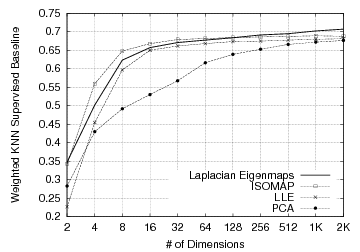
\includegraphics[width=0.5\textwidth]{baseline_graph_mono.png}
\caption{Supervised knn baselines for the four dimensionality
  reduction algorithms.}
\label{fig:dimreduce}
\end{figure}

% /scratch/esert/pos_ind/work/BASELINE_GRAPH/plot_data
% dimension PCA    LLE     ISO     LEM(Spectral)
% 2              0.2831 0.2272 0.3433 0.3480
% 4              0.4300 0.4547 0.5596 0.5019
% 8              0.4920 0.5968 0.6480 0.6234
% 16            0.5303 0.6500 0.6678 0.6572
% 32            0.5676 0.6617 0.6790 0.6708
% 64            0.6162 0.6680 0.6818 0.6774
% 128          0.6390 0.6735 0.6844 0.6838
% 256          0.6527 0.6747 0.6860 0.6914
% 512          0.6658 0.6774 0.6876 0.6948
% 1024        0.6720 0.6798 0.6891 0.7022
% 2048        0.6764 0.6811 0.6878 0.7070
% 

% this should be about same
The graph based algorithms (Isomap, LLE, and Laplacian eigenmaps) all
outperform PCA.  They stay within 5\% of their peak accuracy with as
few as 16 dimensions.  In fact Laplacian eigenmaps outperform the
baseline with the original 12,672 dimensional vectors (68.95\%) when
allowed to retain more than about 250 dimensions.  Spectral clustering
uses the same transformation as the Laplacian eigenmaps algorithm and
we compare its performance to other clustering algorithms in the next
section.

%%

\section{Clustering}
\label{sec:clustering}

We compared three clustering algorithms applied to the original
substitute vectors using many-to-one accuracy on the 45-tag 24K word
test corpus.  Hierarchical agglomerative clustering with complete
linkage (HAC) starts with each instance in its own cluster and
iteratively combines the two closest groups (measured by their most
distant points) at each step \cite{manning2008introduction}.
K-medoids minimizes sum of pairwise distances between each datapoint
to the exemplar at the center of its cluster
\cite{kaufman2005finding}.  Spectral clustering\footnote{We used the
  implementation in \cite{chen2011parallel} with a symmetric sparse
  affinity matrix of 550 nearest neighbors.} uses the eigenvalues of
the graph Laplacian $L=D^{-1/2} W D^{-1/2}$ to reduce the number of
dimensions (similar to Laplacian eigenmaps) and uses simple k-means
clustering on the resulting representation \cite{ng2002spectral}.  All
three algorithms accept the distance matrix based on the KL2 distance
(see Section~\ref{sec:dist}) as input.

\begin{figure}[h]
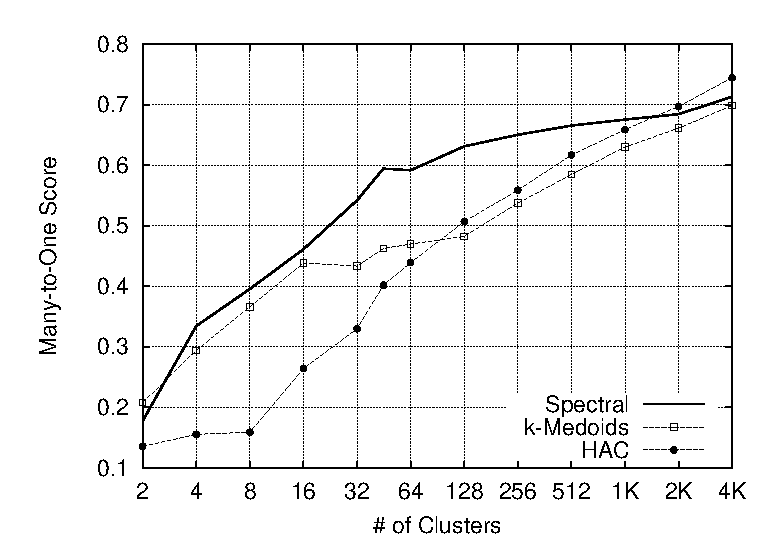
\includegraphics[width=.5\textwidth]{clustering_graph_mono.eps}
\caption{Many-to-one score for three clustering algorithms on the
  45-tag 24K word corpus.}
\label{fig:clustering}
\end{figure}

% #cluster kmedoid spectral hac
% 2          0.20795 0.17781 0.135762
% 4          0.29413 0.33439 0.155579
% 8          0.36615 0.39550 0.159076
% 16        0.43830 0.46116 0.263988
% 32        0.43318 0.54192 0.329850
% 45        0.46245 0.59413 0.401832
% 64        0.46965 0.59151 0.438843
% 128      0.48235 0.63106 0.506703
% 256      0.53709 0.65000 0.558659
% 512      0.58464 0.66520 0.616653
% 1024     0.62985 0.67523 0.658576
% 2048     0.66107 0.68414 0.696878
% 4096     0.69842 0.71286 0.744338


Figure~\ref{fig:clustering} plots the many-to-one score versus number
of clusters for the three algorithms on the 45-tag 24K word test
corpus.  The many-to-one score naturally increases as we approach the
one cluster per word limit, however we find the evolution of the
curves informative.  At the high end (more than 2000 clusters) HAC
performs best with its conservative clusters, but its performance
degrades fast as we reduce the number of clusters because it cannot
reverse the accumulating mistakes.  At the low end (less than 16
clusters) k-medoids and spectral have similar performance.  However
for the region of interest (between 16 to 2000 clusters) spectral
clustering is clearly superior with \spectralResult\% many-to-one
accuracy at 45 clusters.


%\section{Increasing Sparsity}
\label{sec:sparsity}

We noted that the 45 cluster spectral clustering result described in
the previous section assigned many more tags to each word than the
gold standard.  To quantify the difference we used a measure called
tag perplexity defined as follows:

\[ 2^{\frac{1}{N}\sum_{i=1}^N -\log_2 p(t_i | w_i)} \]

Here $N$ is the number of words in the corpus, $w_i$ is the i'th word,
$t_i$ is its assigned cluster or tag, and $p(t_i|w_i)$ is the fraction
of times word $w_i$ has been assigned $t_i$.  A model which had to
choose from $q$ equally likely tags for each word would have a tag
perplexity of $q$.  The tag perplexity of the gold standard 45-tag 24K
word test corpus is 1.09, whereas the tag perplexity of the spectral
clustering result is 2.76.

We experimented with two methods for reducing the number of tags
assigned to each word: collapsing and word penalties.  Collapsing
enforces the one-tag-per-word constraint by re-tagging the corpus,
whereas word penalties encourage it by increasing the distance between
instances with different target words.

To collapse a given tag assignment for a corpus, we re-tag each word
with its most frequent tag in the original assignment (we break ties
randomly).  This forcefully reduces the tag perplexity to 1 and
removes any ambiguity.  Collapsing improves the many-to-one accuracy
by more than 10\% from \spectralResult\% to \collapseResult\%.

Interestingly when we try to enforce the one-tag-per-word restriction
before clustering (by giving the average substitute vector for each
word type to spectral clustering) the results get worse (58.02\%
many-to-one accuracy).  The information in individual instances seems
to be necessary for good clusters to arise.

Word penalties include information about the target word in the
distance metric.  The substitute vectors and the KL2 distance metric
based on them carry no information about the target word, only its
context.  We used the following distance metric which increases the
distance between instances with different target words:

\[ D(i, j) = KL2(s_i,s_j)+\delta I(w_i \neq w_j) \]

Here $s_i$ is the substitute vector and $w_i$ is the target word for
the i'th position, $\delta$ is the regularization parameter, and $I$
is the indicator function that gives 1 if the two words are different
and 0 if they are the same.  Increasing the $\delta$ decreases the tag
perplexity, but the accuracy change is non-monotonic.  At $\delta=1$
we obtain a tag perplexity of 1.91 and the many-to-one accuracy
increases from \spectralResult\% to 64.35\%.  This demonstrates that
we can significantly increase the accuracy by including more
information on the target word without employing the full
one-tag-per-word constraint.  
%% Table~\ref{tab:results} summarizes the results.

%% % do we need graph of delta vs accuracy? no does not look meaningful.

%% \begin{table}[h] \centering
%% \begin{tabular}{|lll|} \hline
%% algorithm & many-1 & tag-perp. \\ \hline
%% spectral & \spectralResult & 2.76 \\
%% word-penalty & 64.35 & 1.91 \\
%% collapsed & \collapseResult & 1.00 \\ \hline
%% gold & 100 & 1.09 \\ \hline
%% \end{tabular}
%% \caption{The many-to-one accuracy and tag perplexity of spectral
%%   clustering, word-penalty, and collapsed algorithms in comparison to
%%   the gold standard.}
%% \label{tab:results}
%% \end{table}

\begin{figure*}[t]
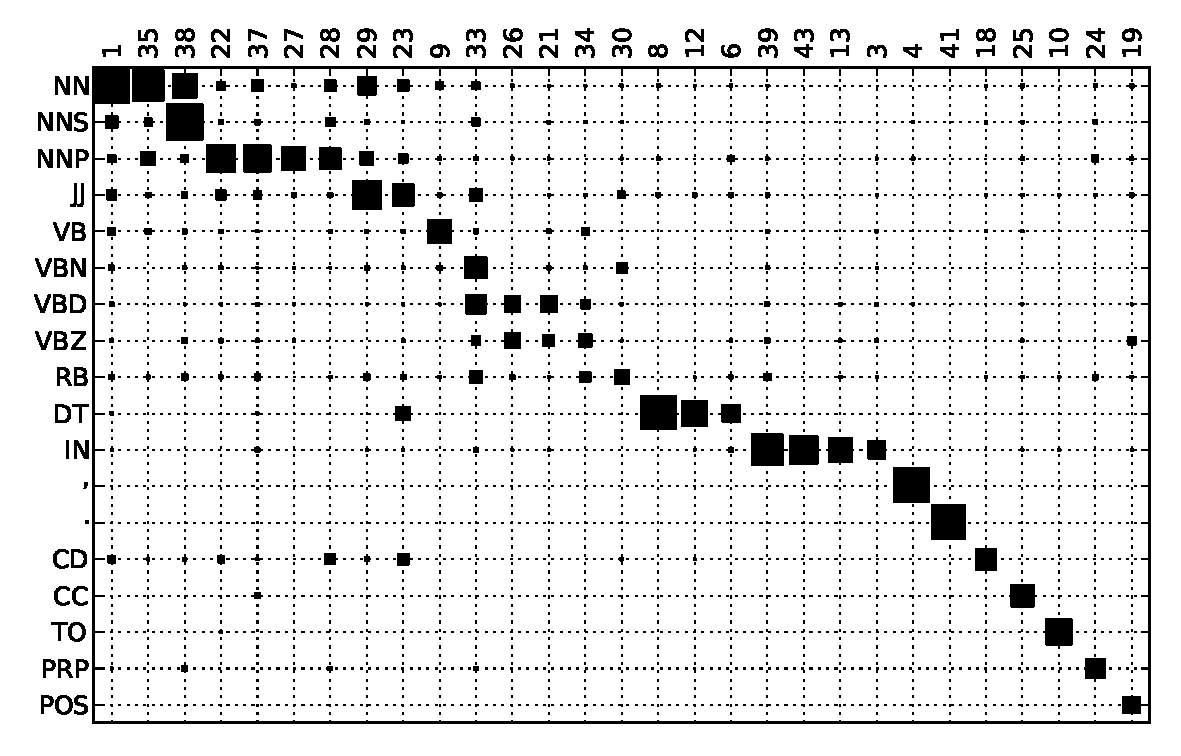
\includegraphics[width=\textwidth]{hinton.eps}
\vspace*{-10mm}
\caption{Hinton diagram of the most frequent tags (rows) and clusters
  (columns).  Area of each square is proportional to the joint
  probability of the given tag and cluster.}
\label{fig:hinton}
\end{figure*}
 % omit
\section{Co-occurrence Data Embedding}
\label{sec:code}

The general strategy we follow for unsupervised syntactic category
acquisition is to combine features of the context with the identity
and features of the target word.  Our preliminary experiments
indicated that using the context information alone (e.g. clustering
substitute vectors) without the target word identity and features had
limited success.\footnote{A 10-nearest-neighbor supervised baseline
  using cosine distance between substitute vectors gives .7213
  accuracy.  Clustering substitute vectors using various distance
  metrics and dimensionality reduction methods give results inferior
  to this upper bound.} It is the co-occurrence of a target word with a
particular type of context that best predicts the syntactic category.
In this section we review the unsupervised methods we used to model
co-occurrence statistics: the Co-occurrence Data Embedding (CODE)
method \cite{globerson2007euclidean} and its spherical extension
(S-CODE) introduced by \cite{maron2010sphere}.

Let $X$ and $Y$ be two categorical variables with finite cardinalities
$|X|$ and $|Y|$.  We observe a set of pairs $\{x_i, y_i\}_{i=1}^n$
drawn IID from the joint distribution of $X$ and $Y$.  The basic idea
behind CODE and related methods is to represent (embed) each value of
$X$ and each value of $Y$ as points in a common low dimensional
Euclidean space $\mathbf{R}^d$ such that values that frequently
co-occur lie close to each other.  There are several ways to formalize
the relationship between the distances and co-occurrence statistics, in
this paper we use the following:
\begin{equation} \label{eq:probability}
p(x,y) = \frac{1}{Z} \bar{p}(x) \bar{p}(y) e^{-d^2_{x,y}}
\end{equation}
\noindent where $d^2_{x,y}$ is the squared distance between the
embeddings of $x$ and $y$, $\bar{p}(x)$ and $\bar{p}(y)$ are empirical
probabilities, and $Z=\sum_{x,y} \bar{p}(x) \bar{p}(y) e^{-d^2_{x,y}}$ is
a normalization term.  If we use the notation $\phi_x$ for the
point corresponding to $x$ and $\psi_y$ for the point corresponding
to $y$ then $d^2_{x,y} = \|\phi_x-\psi_y\|^2$.  The log-likelihood
of a given embedding $\ell(\phi, \psi)$ can be expressed as:
\begin{eqnarray} 
&&\ell(\phi, \psi) = \sum_{x,y} \bar{p}(x,y) \log p(x,y) \label{eq:likelihood} \\
&&= \sum_{x,y} \bar{p}(x,y) (-\log Z + \log \bar{p}(x)\bar{p}(y) - d^2_{x,y}) \nonumber \\
&&= -\log Z + \mathit{const} - \sum_{x,y} \bar{p}(x,y) d^2_{x,y} \nonumber
\end{eqnarray}
The likelihood is not convex in $\phi$ and $\psi$.  We use gradient
ascent to find an approximate solution for a set of $\phi_x$, $\psi_y$
that maximize the likelihood.  The gradient of the $d^2_{x,y}$ term
pulls neighbors closer in proportion to the empirical joint
probability:
\begin{equation}
\frac{\partial}{\partial\phi_x} \sum_{x,y} -\bar{p}(x,y) d^2_{x,y} =
\sum_y 2 \bar{p}(x,y) (\psi_y - \phi_x) \label{eq:attract}
\end{equation}
The gradient of the $Z$ term pushes neighbors apart in proportion to the
estimated joint probability:
\begin{equation}
\frac{\partial}{\partial\phi_x} (-\log Z) = \sum_y 2 p(x,y) (\phi_x -
\psi_y) \label{eq:repulse}
\end{equation}
Thus the net effect is to pull pairs together if their estimated
probability is less than the empirical probability and to push them
apart otherwise.  The gradients with respect to $\psi_y$ are
similar.

S-CODE \cite{maron2010sphere} additionally restricts all $\phi_x$ and
$\psi_y$ to lie on the unit sphere.  With this restriction, $Z$ stays
around a fixed value during gradient ascent.  This allows S-CODE to
substitute an approximate constant $\tilde{Z}$ in gradient
calculations for the real $Z$ for computational efficiency.  In our
experiments, we used S-CODE with its sampling based stochastic
gradient ascent algorithm and smoothly decreasing learning
rate.


%\subsection{S-Code and Substitute Vector Application}
\subsection{Experimental Settings}\label{sec:expset}

To make a meaningful comparison on the PTB we ran all the experiments
using the following default settings (unless otherwise stated): (i)
each word was kept with its original capitalization, (ii) the learning
rate parameters were set to $\varphi_0=50$, $\eta_0=0.2$ for faster
convergence in log likelihood, (iii) the number of S-CODE iterations
were set to 50 million, (iv) the S-CODE dimensions and $Z$ were set to
25 and 0.166, respectively, (v) a modified k-means algorithm with
smart initialization was used \cite{arthur2007k}, and (vi) the number
of k-means restarts were set to 128 to improve clustering and reduce
variance.

Section~\ref{sec:dist} shows that low probability substitutes are
relatively unimportant thus for computational efficiency only the top
100 substitutes and their unnormalized probabilities were computed for
each positions in the PTB(1,173,766 tokens, 49,206 types) using the
{\sc fastsubs} algorithm \cite{yuret2021fastsub}\footnote{The
  substitutes with unnormalized log probabilities can be downloaded
  from \mbox{\url{http://goo.gl/jzKH0}}.}.  The probability vectors
for each position were normalized to add up to 1.0 giving us the final
substitute vectors used in the rest of this study.  We set the
vocabulary threshold to 20 which increases the vocabulary size to
78,498.

% \footnote{Reducing the vocabulary threshold to 20 from 500

%  increases the vocabulary size to 78,498 from 12,672. }

Each experiment was repeated 10 times with different random seeds and
the results are reported with standard errors in parentheses or error
bars in graphs.  Table~\ref{tab:results} summarizes all the results
reported in this section and the ones we cite from the literature.

\subsection{Random Partitions}\label{sec:rpart}
\begin{table*}[t] \footnotesize
\caption{Summary of results in terms of the \mto and \vm scores.
  Standard errors are given in parentheses when available.  Starred
  entries have been reported in the review paper
  \protect\cite{Christodoulopoulos:2010:TDU:1870658.1870714}.  Distributional
  models use only the identity of the target word and its context.
  The models on the right incorporate orthographic and
  morphological features.}
\begin{tabular}{|@{ }l@{ }|@{ }l@{ }|@{ }l@{ }|}
\hline
Distributional Models & \mto & \vm \\
\hline
Lamar et al. \shortcite{Lamar:2010:LCU:1870658.1870736} & .708 & -\\ %algorithm name LDC
Brown et al. \shortcite{Brown:1992:CNG:176313.176316}* & .678 & .630\\
%kcls(Och,1999) & .737 & .656\\
%\cite{goldwater-griffiths:2007:ACLMain} & .632 & .562\\
Goldwater et al. \shortcite{goldwater-griffiths:2007:ACLMain} & .632 & .562\\
Ganchev et al. \shortcite{Ganchev:2010:PRS:1859890.1859918}* & .625 & .548\\
Maron et al. \shortcite{maron2010sphere} & .688 (.0016)&-\\
Bigrams (Sec.~\ref{sec:bigram}) & \bgmto & \bgvm \\
Partitions (Sec.~\ref{sec:rpart}) & \rpmto & \rpvm \\
Substitutes (Sec.~\ref{sec:wordsub}) & \wsmto & \wsvm \\
\hline
\end{tabular}
\begin{tabular}{|@{ }l@{ }|@{ }l@{ }|@{ }l@{ }|}
\hline
Models with Additional Features & \mto & \vm \\
\hline
Clark \shortcite{Clark:2003:CDM:1067807.1067817}* & .712 & .655 \\
Christodoulopoulos et al. \shortcite{christodoulopoulos-goldwater-steedman:2011:EMNLP} & .728 & .661\\
Berg-Kirkpatrick et al. \shortcite{bergkirkpatrick-klein:2010:ACL} & .755 & -\\ % Interesting in  christo paper:73.9/67.7
Christodoulopoulos et al. \shortcite{Christodoulopoulos:2010:TDU:1870658.1870714} & .761 & .688\\
Blunsom and Cohn \shortcite{blunsom-cohn:2011:ACL-HLT2011} & .775 & .697\\
Substitutes and Features (Sec.~\ref{sec:feat}) & \ftmto & \ftvm \\
& & \\
& & \\
\hline
\end{tabular}
\label{tab:results}
\end{table*}

To obtain a discrete representation of the context, the
random--partitions algorithm first designates a random subset of
substitute vectors as centroids to partition the space, and then
associates each context with the partition defined by the closest
centroid in cosine distance.  Each partition thus defined gets a
unique id, and word ($X$) -- partition-id ($Y$) pairs are given to
S-CODE as input.  The algorithm uses stochastic gradient ascent to
find the $\phi_x, \psi_y$ embeddings for word and partition-id in
these pairs on a single 25-dimensional sphere.  The algorithm cycles
through the data until we get approximately 50 million updates.  The
resulting $\phi_x$ vectors are clustered using an instance weighted
k-means algorithm and the resulting groups are compared to the correct
part-of-speech tags.  Using default settings with 64K random
partitions the many-to-one accuracy is \rpmto\ and the V-measure is
\rpvm.

To analyze the sensitivity of this result to our specific parameter
settings we ran a number of experiments where each parameter was
varied over a range of values.

\begin{figure}[ht] \centering
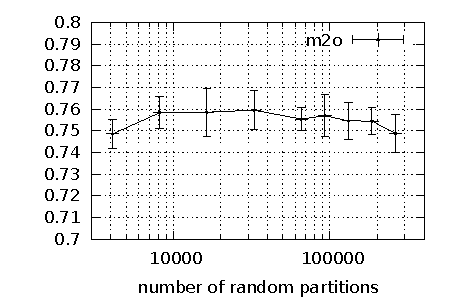
\includegraphics[width=0.5\linewidth]{plot-p.pdf}
\caption{\mto is not sensitive to the number of partitions used to
  discretize the substitute vector space within our experimental
  range.}
\label{plot-p}
\end{figure}

Figure~\ref{plot-p} gives results where the number of initial random
partitions is varied over a large range and shows the results to be
fairly stable across two orders of magnitude.

\begin{figure}[ht] \centering
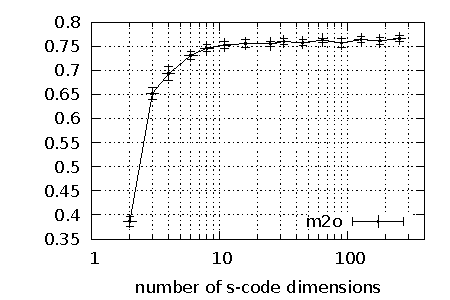
\includegraphics[width=0.5\linewidth]{plot-d.pdf}
\caption{\mto falls sharply for less than 10 S-CODE dimensions, but
  more than 25 do not help.}
\label{plot-d}
\end{figure}

Figure~\ref{plot-d} shows that at least 10 embedding dimensions are
necessary to get within 1\% of the best result, but there is no
significant gain from using more than 25 dimensions.

\begin{figure}[ht] \centering
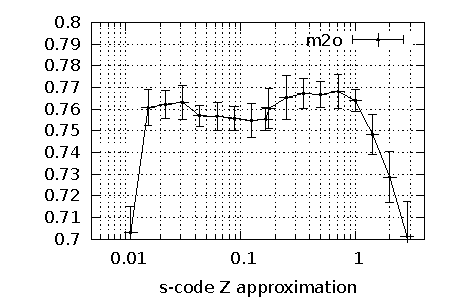
\includegraphics[width=0.5\linewidth]{plot-z.pdf}
\caption{\mto is fairly stable as long as the $\tilde{Z}$ constant is
  within an order of magnitude of the real $Z$ value.}
\label{plot-z}
\end{figure}

Figure~\ref{plot-z} shows that the constant $\tilde{Z}$ approximation
can be varied within two orders of magnitude without a significant
performance drop in the many-to-one score.  For uniformly distributed
points on a 25 dimensional sphere, the expected $Z\approx 0.146$.  In
the experiments where we tested we found the real $Z$ always to be in
the 0.140-0.170 range.  When the constant $\tilde{Z}$ estimate is too
small the attraction in Eq.~\ref{eq:attract} dominates the repulsion
in Eq.~\ref{eq:repulse} and all points tend to converge to the same
location.  When $\tilde{Z}$ is too high, it prevents meaningful
clusters from coalescing.
%%% I have seen the first, but the second is pure guess, need to
%%% look.  The distances seem to be decreasing on that end as well!

We find the random partition algorithm to be fairly robust to
different parameter settings and the resulting many-to-one score
significantly better than the state-of-the-art distributional models.

\subsection{Random Substitutes}\label{sec:wordsub}

Another way to use substitute vectors in a discrete setting is simply
to sample individual substitute words from them according to the
corresponding probabilities.  The random-substitutes algorithm cycles
through the test data and pairs each word with a random substitute
picked from the pre-computed substitute vectors (see
Section~\ref{sec:subthr}).  We ran the random-substitutes algorithm to
generate 76 million word ($X$) -- random-substitute ($Y$) pairs (64
substitutes for each token) as input to S-CODE.  Clustering the
resulting $\phi_x$ vectors yields a many-to-one score of \wsmto\ and a
V-measure of \wsvm.

This result is close to the previous result by the random-partition
algorithm, \rpmto, demonstrating that two very different discrete
representations of context based on paradigmatic features give
consistent results.  Figure~\ref{plot-s} illustrates that the
random-substitute result is fairly robust as long as the training
algorithm can observe more than a few random substitutes per word.

\begin{figure}[ht] \centering
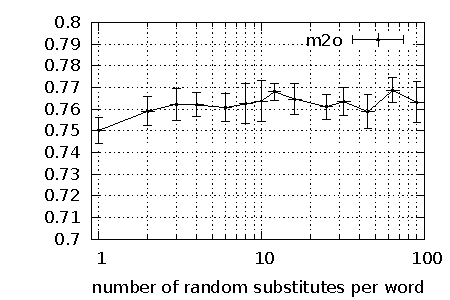
\includegraphics[width=0.5\linewidth]{plot-s.pdf}
\caption{\mto is not sensitive to the number of random substitutes
  sampled per word token.}
\label{plot-s}
\end{figure}

\subsection{Paradigmatic vs Syntagmatic Representations of Word Context}\label{sec:bigram}

To get a direct comparison of the paradigmatic and syntagmatic context
representations we feed the adjacent word pairs (bigrams) in the
corpus into the S-CODE algorithm as $X, Y$ samples
\cite{maron2010sphere} instead of pairing each word with a
paradigmatic representation of its context.  At the end each word $w$
in the vocabulary ends up with two points on the sphere, a $\phi_w$
point representing the behavior of $w$ as the left word of a bigram
and a $\psi_w$ point representing it as the right word.  The two
vectors for $w$ are concatenated to create a 50-dimensional
representation at the end.  These 50-dimensional vectors are clustered
using the k-means algorithm.  Maron et al. \shortcite{maron2010sphere}
report many-to-one scores of .6880 (.0016) for 45 clusters and .7150
(.0060) for 50 clusters (on the PTB).  If only $\phi_w$ vectors are
clustered without concatenation we found the performance drops
significantly to about .62.  Using our default settings the bigram
model achieves \bgmto \mto and \bgvm \vm accuracies.  Both results are
significantly lower than the random partition and substitute \mto and
\vm accuracies.

\section{Multiple Languages}
\begin{landscape}
%%Multiple laguage section
\begin{table}[ht]
  \begin{tabular}{|l|l|l|p{2cm}|p{2cm}|p{2cm}|p{2cm}|p{2cm}|p{2cm}|p{2cm}|}
        \hline
        Language   & Types   & Tags & k-means      & SVD2         & clark        & BMMM         & PYP-1HMM-LM & uPos Letter Features & uPos     \\ \hline % Multext data
        English    & 49,190  & 45   & 59.5 / 61.6   & 58.2 / 64.0   & 65.6 / 71.2   & 66.1 / 72.8   & 69.7 / 77.5 & ~               & \wsvm / \wsmto           \\ \hline
        Bulgarian  & 16,352  & 12+1 & 50.3 / 59.3   & 41.7 / 51.0   & 55.6 / 66.5   & 54.5 / 64.4   & -           & 55.1 / 70.7     & 53.3 / 69.4 \\
        Czech      & 19,115  & 12+1 & 48.6 / 56.7   & 35.5 / 50.9   & 52.6 / 64.1   & 53.9 / 64.2   & -           & 47.9 / 67.0     & 47.2 / 66.9 \\
        English    & 9,773   & 12+1 & 56.5 / 65.4   & 52.3 / 65.5   & 60.5 / 70.6   & 63.3 / 73.3   & -           & 67.1 / 82.9     & 66.6 / 83.2 \\
        Estonian   & 17,845  & 12+1 & 45.3 / 55.6   & 38.7 / 55.3   & 44.4 / 58.4   & 53.3 / 64.4   & -           & 44.9 / 65.4     & 43.4 / 65.1 \\
        Hungarian  & 20,321  & 11+1 & 46.7 / 53.9   & 39.8 / 49.5   & 48.9 / 61.4   & 54.8 / 68.2   & -           & 51.9 / 70.2     & 49.6 / 68.6 \\
        Romanian   & 15,189  & 12+1 & 45.2 / 55.1   & 42.1 / 52.6   & 40.9 / 49.9   & 52.3 / 61.1   & -           & 51.9 / 65.9     & 49.5 / 64.3 \\
        Slovene    & 17,871  & 12+1 & 46.9 / 56.2   & 39.5 / 54.2   & 54.9 / 69.4   & 56.7 / 67.9   & -           & 49.1 / 69.2     & 47.4 / 68.0 \\
        Serbian    & 18,095  & 12+1 & 41.4 / 47.0   & 39.1 / 54.6   & 51.0 / 64.1   & 49.0 / 62.0   & -           & 43.7 / 61.3     & 44.4 / 62.4 \\
        Arabic     & 12,915  & 20   & 43.3 / 60.7   & 27.6 / 49.0   & 40.6 / 59.8   & 42.4 / 61.5   & - / 67.5    & -               & -           \\ \hline % Conll06 data
        Bulgarian  & 32,439  & 54   & 53.6 / 65.6   & 49.0 / 65.3   & 59.6 / 70.4   & 58.8 / 68.9   & - / 73.2    & 57.9 / 73.4     & 57.5 / 73.2 \\
        Chinese    & 40,562  & 15   & 32.6 / 61.1   & 24.5 / 54.6   & 31.8 / 56.7   & 42.6 / 69.4   & -           & -               & -           \\
        Czech      & 130,208 & 12   & -             & -            & 47.1 / 65.5   & 48.4 / 65.7    & - / 70.1    & 53.3 / 72.1     & 48.4 / 67.4 \\
        Danish     & 18,356  & 25   & 51.7 / 61.6   & 40.8 / 57.6   & 52.7 / 65.3   & 59.0 / 71.1   & - / 76.2    & 59.3 / 75.2     & 54.9 / 71.6 \\
        Dutch      & 28,393  & 13   & 45.3 / 60.5   & 36.7 / 52.4   & 52.2 / 67.9   & 54.7 / 71.1   & - / 70.4    & 59.5 / 73.8     & 53.6 / 69.7 \\
        German     & 72,326  & 54   & 58.7 / 67.5   & 54.1 / 64.2   & 63.0 / 73.9   & 61.9 / 74.4   & -           & 65.2 / 76.9     & 62.7 / 76.0 \\
        Japanese   & 3,231   & 80   & 76.1 / 76.2   & 74.4 / 75.5   & 78.6 / 77.4   & 77.4 / 78.5   & -           & -               & -           \\
        Portuguese & 28,931  & 22   & 51.6 / 64.4   & 45.9 / 63.1   & 57.4 / 69.2   & 63.9 / 76.8   & - / 78.5    & 61.9 / 77.5     & 57.2 / 73.6 \\
        Slovene    & 7,128   & 29   & 52.6 / 64.2   & 44.0 / 60.3   & 53.9 / 63.5   & 49.4 / 56.2   & -           & 49.6 / 64.8     & 48.2 / 64.2 \\
        Spanish    & 16,458  & 47   & 59.5 / 69.2   & 54.8 / 68.2   & 61.6 / 71.9   & 63.2 / 71.7   & - / 78.8    & 63.3 / 76.8     & 60.2 / 74.4 \\
        Swedish    & 20,057  & 41   & 53.2 / 62.2   & 47.4 / 59.1   & 58.9 / 68.7   & 58.0 / 68.2   & - / 68.6     & 56.9 / 69.2      & 56.2 / 69.2 \\
        Turkish    & 17,563  & 30   & 40.8 / 62.8   & 27.4 / 52.4   & 36.8 / 58.1   & 40.2 / 58.7   & -           & re-run          & 36.8 / 61.3  \\ \hline % extra data from cristo2011 paper
        French     & 49,964  & 23   & 48.2 / 68.6   & 46.3 / 68.5   & 57.3 / 77.8   & 55.0 / 76.6   & -           & -               & -        \\
        A.Greek    & 15,194  & 15   & 38.6 / 44.8   & 24.2 / 38.5   & 33.3 / 45.4  & 40.5 / 45.1    & -           & -               & -        \\ \hline
    \end{tabular}
\end{table}
\end{landscape}

\section{Discussion}
\label{sec:discussion}

Figure~\ref{fig:hinton} is the Hinton diagram showing the relationship
between the most frequent tags and clusters found by the collapsed
algorithm (\collapseResult\% many-to-one accuracy).  In this section
we present a qualitative comparison of gold standard tags and
discovered clusters.

\paragraph{Nouns and adjectives:} Most nouns ({\sc nn*}) are split between the
clusters represented by the first seven columns of the Hinton graph,
but not in the way Penn Treebank splits them.  For example cluster 27
brings together titles like {\em Mr.}, {\em Mrs.}, {\em Dr.}
etc. which does not exist as a separate class in the gold tags.
Cluster 29 is the largest adjective ({\sc jj}) cluster, however it
also has noun members probably due to the difficulty of separating
noun-noun compounds and adjective modification.

\paragraph{Verbs and adverbs:}  Clusters 9 and 33 contain general
verbs ({\sc vb*}), but the verbs ``be'' (26), ``say'' (21), and
``have'' (34) have been split into their own clusters indicated in
parantheses, presumably because they are not generally substitutable
with the rest.  Adverb ({\sc rb}) is an amorphous class and the
algorithm seems to have difficulty isolating it in a cluster.

\paragraph{Determiners and prepositions:}  We see a fairly clean
separation of determiners ({\sc dt}) and prepositions ({\sc in}) from
other parts of speech, although each has been subdivided into further
groups by the algorithm.  For example cluster 39 contains general
prepositions but ``of'' (43), ``in'' (13), and ``for'' (3) are split
into their own clusters.  Determiners ``the'' (8), ``a'' (12), and
capitalized ``The''/''A'' (6) are also split into their own clusters.

\paragraph{Closed-class items:}  Most closed-class items are cleanly
separated into their own clusters as seen in the lower right hand
corner of the diagram.

\section{Contributions}
\label{sec:contrib}

Our main contributions can be summarized as follows:
\begin{itemize}
\item We introduced substitute vectors as paradigmatic representations
  of word context and demonstrated their use in unsupervised part of
  speech induction on 19 corpora in 15 languages.
\item We demonstrated that using paradigmatic representations of word
  context and modeling co-occurrences of word and context types with
  the S-CODE learning framework give superior results when compared to
  a syntagmatic bigram model.
\item We extended the S-CODE framework to incorporate morphological
  and orthographic features and improved the state-of-the-art
  many-to-one accuracy in unsupervised part of speech induction on 17
  out of 19 corpora.
\item All our code and data, including the substitute vectors for the
  PTB, MULTEXT-East and CoNLL-X shared task corpora are available
  at the authors' website at \mbox{\url{xxx.xxx.xxx}}.
\end{itemize}



\bibliographystyle{colin}
\bibliography{posind2012}

\end{document}
